\documentclass[tikz]{standalone}
\usepackage{tikz-network}
\begin{document}

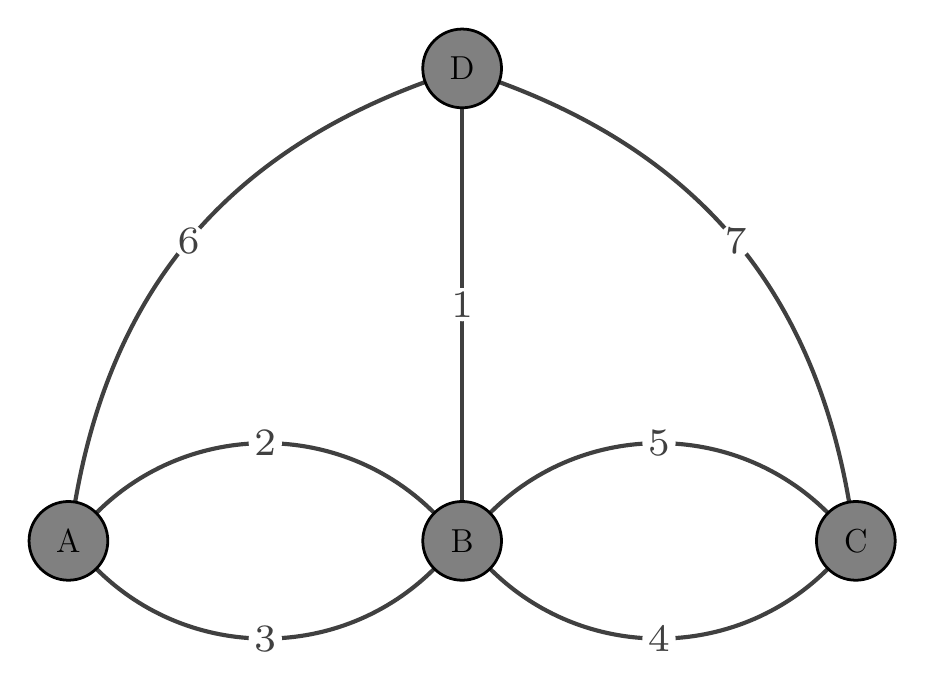
\begin{tikzpicture}
\Vertex[IdAsLabel, x=5, color=gray, size=1, fontsize=\large]{A}
\Vertex[IdAsLabel, x=10, color=gray, size=1, fontsize=\large]{B}
\Vertex[IdAsLabel, x=15, color=gray, size=1, fontsize=\large]{C}
\Vertex[IdAsLabel, x=10, y=6, color=gray, size=1, fontsize=\large]{D}

\Edge[label=2, bend=45, fontscale=2](A)(B)
\Edge[label=6, bend=30, fontscale=2](A)(D)
\Edge[label=3, bend=45, fontscale=2](B)(A)
\Edge[label=5, bend=45, fontscale=2](B)(C)
\Edge[label=4, bend=45, fontscale=2](C)(B)
\Edge[label=7, bend=30, fontscale=2](D)(C)
\Edge[label=1, fontscale=2](D)(B)
\end{tikzpicture}
\end{document}
